% Drawing 57/07-1 -- folder 57, batch 07, archive page 122 (PDF page 123).
% Transcription: figure : les composantes $X_i$, $X_j$ découpées dans $X$ par des arcs, $Y_i$ et $Y_j$ portés sur elles, $X_{ij}$ et $Z_{ij}$ marqués au point d'intersection, avec flèches vers les étiquettes
% Kind: components of a scheme cut by arcs. Method 2 (schematic redraw from the facsimile). Status: ok.
% Notes: Strokes meeting at one computed point each: the heavy point P, from which run the short strokes to the left and to the lower right, the stroke down to the lower left corner C1, the arc coming from the upper left (Y_i side), the long curve to the upper right and the stroke to the right towards the label Y_j; from C1 the lower arc to the right corner R1 (which rises to the top right) and the curve down to the bottom; the long stroke from the top crossing everything down to its corner K, which turns back to the lower left; the separate line at the upper left. On the right, the heavy vertical stroke and the narrow wedge. Arrows: the curved arrow from X, the arrows towards P from Y_i, from X_ij down to the crossing, the arrowhead before Y_j, the arrow from the right. Labels at \small after the transcription, where the letters stand: X, Y_i, X_ij, Y_j, Z_ij, and "ij)" under P. Still differs: which piece is X_i and which X_j cannot be told, so neither is written; the reading of the two right-hand labels (Y_j, Z_ij) and of the top left X (perhaps X_i) follows the earlier redraw and the transcription, not a clear reading of the page; the heavy vertical on the right may be part of a label. Redrawn 2026-11-09 (issue 128): to check again. Revised 2026-11-09 after Michel's check (#135): yes, the labels are right as drawn (X, Y_i, X_ij, Y_j, Z_ij, ij)), after the transcription; ok.
% Coordinates: 1 unit = 1 mm = 1/100 of the crop width (bbox in page fractions: [0.11, 0.28, 0.33, 0.43]).
% Redrawn by Claude (claude-opus-5-5), issue #73, 2026-11-09; not checked by a human; not compiled (no TeX in the session).
% Rights: reproduces part of the work -- behind RENDER_TRANSCRIPTS, never published by itself.
\documentclass[tikz,border=3pt]{standalone}
\usepackage{amsmath,amssymb}
\usetikzlibrary{patterns,arrows.meta}
\tikzset{pencil/.style={black!45}, struck/.style={black!35}, mark/.style={circle,draw,inner sep=1.3pt}, pt/.style={circle,fill,inner sep=0.9pt}, opt/.style={circle,draw,fill=white,inner sep=1.1pt}}
\begin{document}
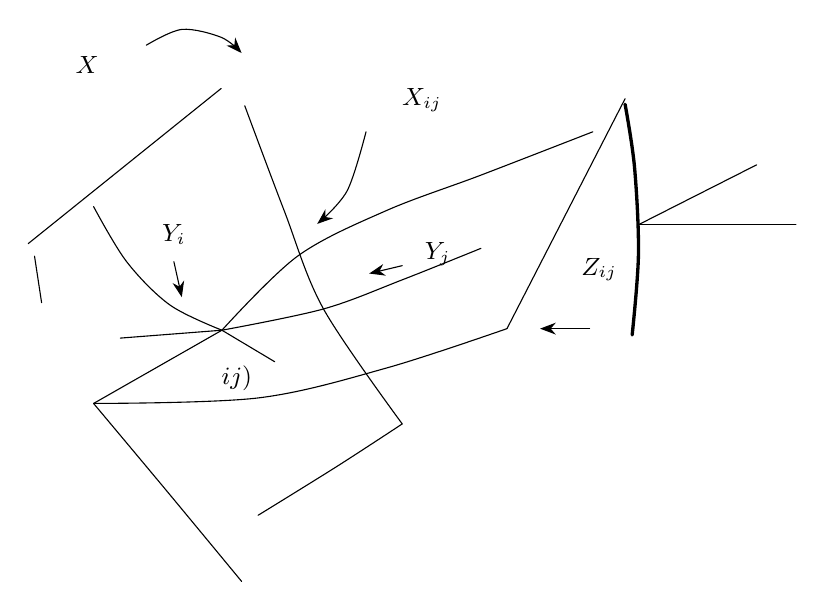
\begin{tikzpicture}[x=1mm,y=1mm,line cap=round,line join=round,font=\scriptsize]
\draw (14.2,-53.7) -- (27.1,-52.7);
\draw (27.1,-52.7) -- (33.8,-56.7);
\draw (27.1,-52.7) -- (10.8,-62);
\draw plot[smooth, tension=0.55] coordinates {(10.8,-37) (15,-44) (20.5,-49.5) (27.1,-52.7)};
\draw plot[smooth, tension=0.55] coordinates {(27.1,-52.7) (36.7,-43.3) (48,-37.5) (60,-33) (74.2,-27.5)};
\draw plot[smooth, tension=0.55] coordinates {(27.1,-52.7) (40,-50) (50,-46.3) (60,-42.3)};
\draw plot[smooth, tension=0.55] coordinates {(10.8,-62) (31.7,-61.3) (48,-57.5) (63.3,-52.5)};
\draw (63.3,-52.5) -- (78.3,-23.3);
\draw plot[smooth, tension=0.55] coordinates {(10.8,-62) (20,-73) (29.6,-84.6)};
\draw plot[smooth, tension=0.55] coordinates {(30,-24.2) (35,-37.5) (40,-50) (50,-64.6)};
\draw plot[smooth, tension=0.55] coordinates {(50,-64.6) (41.7,-70) (31.7,-76.2)};
\draw (2.5,-41.7) -- (27,-22);
\draw (3.3,-43.3) -- (4.2,-49.2);
\draw[very thick] plot[smooth, tension=0.55] coordinates {(78.3,-24) (79.5,-32) (80,-43) (79.2,-53.3)};
\draw (80,-39.3) -- (95,-31.7);
\draw (80,-39.3) -- (100,-39.3);
\draw[-{Stealth[length=2mm]}] plot[smooth, tension=0.55] coordinates {(17.5,-16.5) (22,-14.5) (27,-15.5) (29.6,-17.5)};
\draw[-{Stealth[length=2mm]}] (21,-44) -- (22,-48.5);
\draw[-{Stealth[length=2mm]}] plot[smooth, tension=0.55] coordinates {(45.4,-27.5) (43,-35) (39.2,-39.2)};
\draw[-{Stealth[length=2mm]}] (50,-44.5) -- (45.8,-45.5);
\draw[-{Stealth[length=2mm]}] (73.8,-52.5) -- (67.5,-52.5);
\node[inner sep=1pt] at (10,-19) {\small $X$};
\node[inner sep=1pt] at (21,-40.5) {\small $Y_i$};
\node[inner sep=1pt] at (52.5,-23.5) {\small $X_{ij}$};
\node[inner sep=1pt] at (54.5,-43) {\small $Y_j$};
\node[inner sep=1pt] at (75,-45) {\small $Z_{ij}$};
\node[inner sep=1pt] at (29,-58.8) {\small $ij)$};
\end{tikzpicture}
\end{document}
